\subsection{Các lực cơ bản}

\begin{frame}
    \frametitle{Lực hấp dẫn}
    \begin{tcolorbox}[colback=blue!10, colframe=blue!50!black, title=Định nghĩa]
    Lực hấp dẫn là lực tương tác giữa hai vật có khối lượng, được mô tả bởi định luật vạn vật hấp dẫn của Newton:
    \begin{equation}
        F = G \frac{m_1 m_2}{r^2}
    \end{equation}
    trong đó \(F\) là lực hấp dẫn, \(G\) là hằng số hấp dẫn, \(m_1\) và \(m_2\) là khối lượng của hai chất điểm, và \(r\) là khoảng cách giữa chúng.
    \end{tcolorbox}
\end{frame}

\begin{frame}
    \frametitle{Lực hấp dẫn}
    \begin{columns}
    \begin{column}{0.5\textwidth}
        \begin{figure}
        \centering
        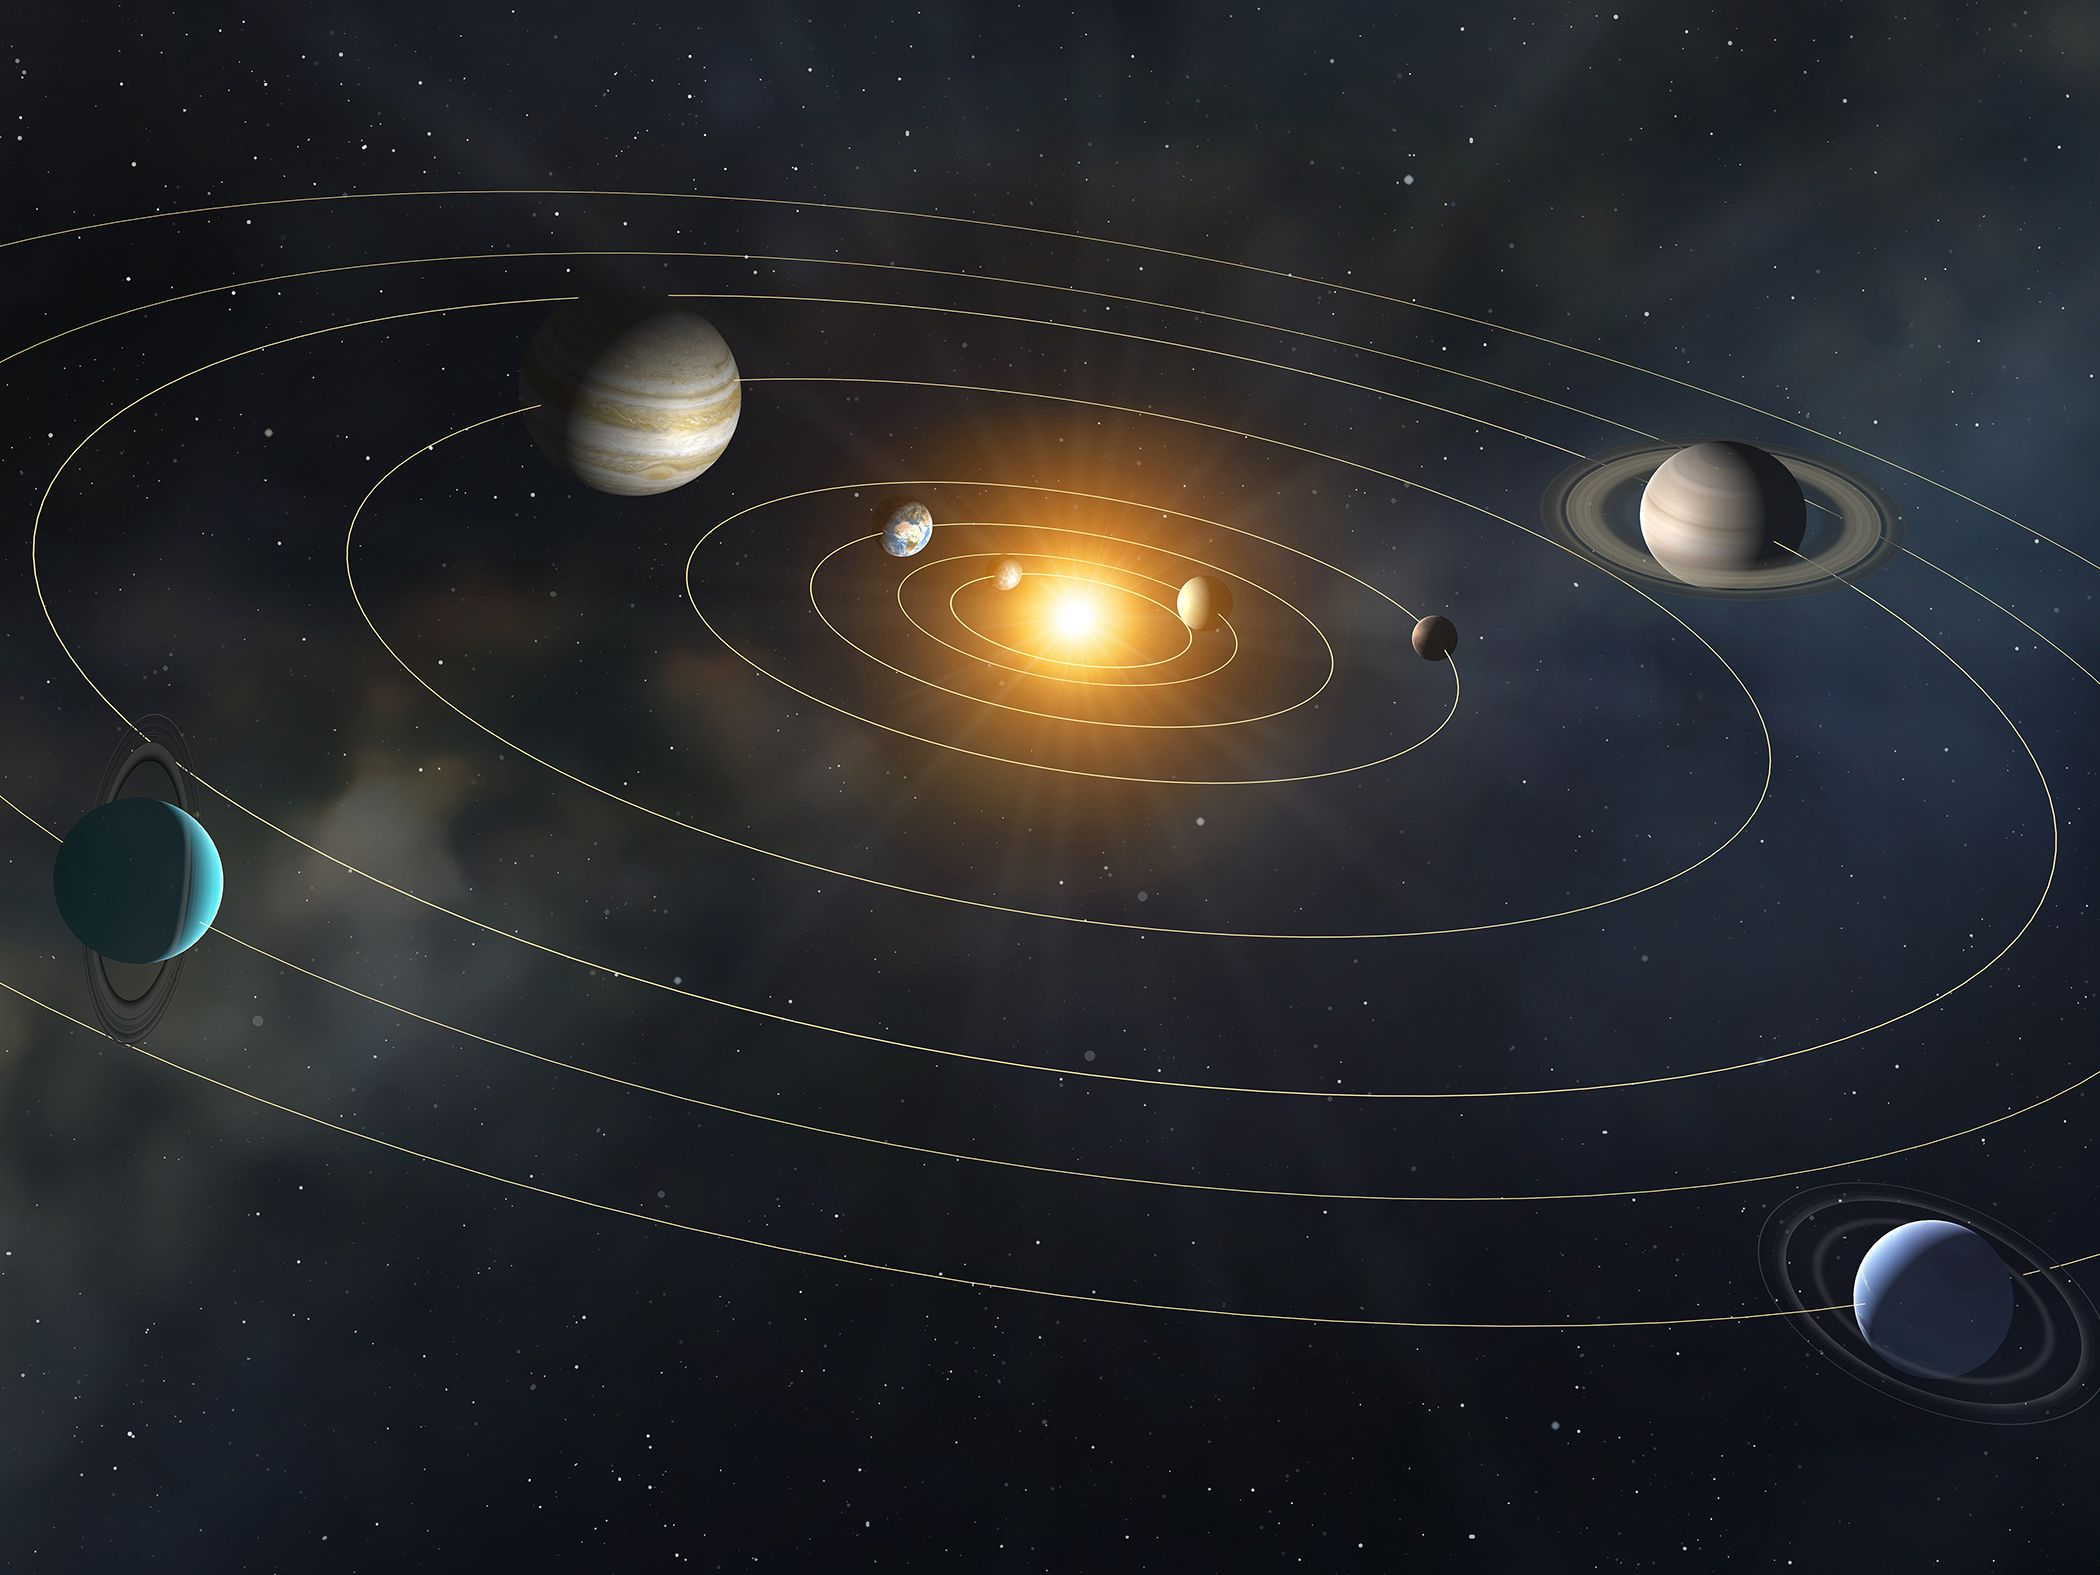
\includegraphics[width=0.8\textwidth]{Slides/Figure/solarsystem.jpg}
        \caption{Các hành tinh quay quanh Mặt Trời}
        \end{figure}
    \end{column}
    \begin{column}{0.5\textwidth}
        \begin{figure}
        \centering
        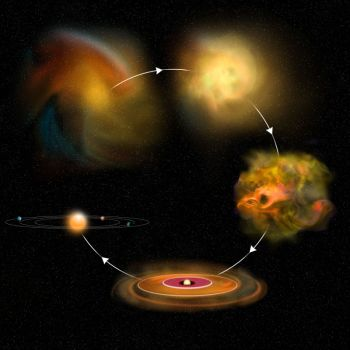
\includegraphics[width=0.6\textwidth]{Slides/Figure/planetformation.jpg}
        \caption{Sự hình thành sao và các hành tinh}
        \end{figure}
    \end{column}
    \end{columns}
\end{frame}

\begin{frame}
    \frametitle{Lực hấp dẫn}
    Ở một nơi trên bề mặt trái đất, trọng lực đối với một vật gần như không đổi, có chiều hướng từ trên xuống dưới mặt đất.
    \begin{columns}
    \begin{column}{0.5\textwidth}
        \begin{figure}
        \centering
        
\includegraphics[width=0.4\textwidth]{Slides/Figure/applefalling.jpg}
        \caption{Quả táo của Newton rơi do trọng lực}
        \end{figure}
    \end{column}
    \begin{column}{0.5\textwidth}
        Lực này có giá trị bằng:
        \begin{equation}
            F=mg
        \end{equation}
        trong đó \(F\) là lực hấp dẫn, \(m\) là khối lượng của vật, và \(g\) là gia tốc trọng trường (khoảng 9.81 m/s² trên bề mặt Trái Đất).
    \end{column}
    \end{columns}
\end{frame}

\begin{frame}
\frametitle{Lực điện từ}
\end{frame}
\subsection{Các lực vĩ mô}
\begin{frame}
    \frametitle{Lực đàn hồi}
\end{frame}
\begin{frame}
    \frametitle{Lực căng}
\end{frame}
\begin{frame}
    \frametitle{Phản lực pháp tuyến}
\end{frame}
\begin{frame}
    \frametitle{Lực ma sát}
\end{frame}